\documentclass[12pt,fleqn]{article}
\setlength{\parindent}{0pt}
\usepackage{graphicx}
\usepackage{cancel}
\usepackage{listings}
\usepackage[latin5]{inputenc}
\usepackage{color}
\setlength{\parskip}{8pt}
\setlength{\parsep}{0pt}
\setlength{\headsep}{0pt}
\setlength{\topskip}{0pt}
\setlength{\topmargin}{0pt}
\setlength{\topsep}{0pt}
\setlength{\partopsep}{0pt}
\setlength{\mathindent}{0cm}
\usepackage{latexsym}
\usepackage{amsfonts}
\usepackage{mathrsfs}
\usepackage{showkeys}
\renewcommand*\showkeyslabelformat[1]{(#1)}

\begin{document}
Ders 24

Green'in Teorisinin iki seklini gormustuk

\[ \oint_C \vec{F} \cdot \vec{T} ds = \int \int_R curl \ \vec{F} \ dA \]

\[ \oint_C \vec{F} \cdot \vec{n} \ ds = \int \int_R div \ \vec{F} \ dA \]


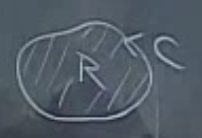
\includegraphics[height=2cm]{24_1.png}

Bu esitliklerin sol tarafi icin $\vec{F}$'in sadece $C$ uzerinde tanimli
olmasi yeterlidir. Fakat esitliklerin anlamli olmasi icin, yani sag
tarafinin da dogru olmasi icin $\vec{F}$'in $R$ icindeki her noktada tanimli
olmasi gerekir. Eger $R$ icinde tanimli olmayan tek bir nokta bile varsa, o
zaman ustteki esitlikleri kullanamayiz.

Ornek 

\[ \vec{F} = \frac{ -y\hat{i} + x\hat{j}}{x^2+y^2} \]

Ustteki $\vec{F}$ orijinde tanimli degildir, diger her yerde , $curl \
\vec{F} = 0$. 
Iki olasiliga bakalim, diyelim ki ``sekilsel'' olarak benzer alanlar orijini
iceren, bir de icermeyen sekillerde verilmis

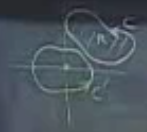
\includegraphics[height=3cm]{24_2.png}

Orijin icermeyen alan icin

\[ \oint_C \vec{F} \cdot d\vec{r} = 
\int \int_R \underbrace{curl \ \vec{F}}_{0} \ dA  = 0
\]
 
Orijin iceren alan icin Green Teori'sini kullanamayiz, cunku cift entegral
icin alan tanimi her yerde tutmali, ama burada alan tanimi orijinde
gecersiz. Ama ``kullanamayiz'' derken aslinda ``direk olarak kullanamayiz''
demek daha dogru olur, dolayli olarak Green Teori'sini kullanmanin bir yolu
var. Tum alan icin olmasa da alanin bir parcasi icin Green Teori'sini
kullanabilirim. 

Eger su alan icin GT kullanamiyorsam

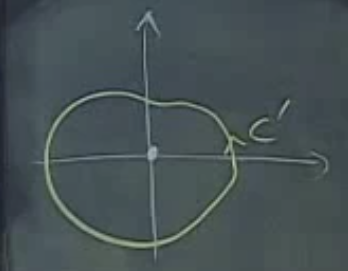
\includegraphics[height=3cm]{24_3.png}

Ustteki bolgenin ortasindaki ufak bir bolgeyi cikartirsam, geri kalan
uzerinde GT kullanabilirim

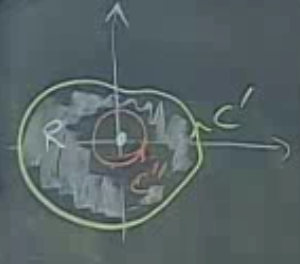
\includegraphics[height=3cm]{24_4.png}


\[ \oint_{C'} \vec{F} \cdot d\vec{r} - 
\oint_{C''} \vec{F} \cdot d\vec{r}  =
\int \int_R curl \ \vec{F} \ dA 
\]
 
Fakat ustteki formulu nasil uygulayacagiz? Soyle bir ek dusunelim, 

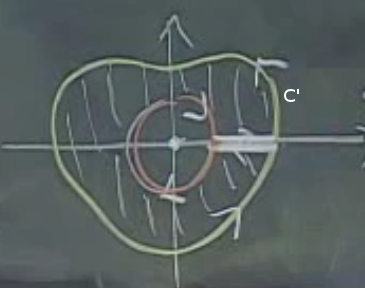
\includegraphics[height=4cm]{24_5.png}

Iki egri arasinda bir ``kopru'' gibi bir gecis noktasi var, bu sonsuz
kucuklukteki bir aralik. Oyle ki bu aralik ile dis egriden ic egriye,
oradan tekrar disari cikiyoruz. Kabaca soyle gosterilebilir (yesil cizgi)

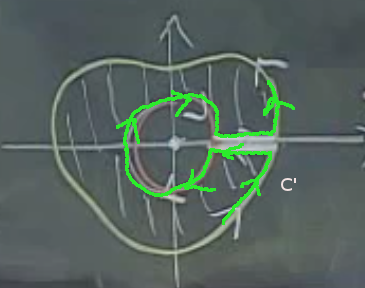
\includegraphics[height=4cm]{24_6.png}

Simdi bu kesintisiz egri uzerinden Green'in Teori'si kullanabilirim, cunku
hem tam bir egri var, hem de tanimsiz olan orijin artik hesaba dahil
degil. 

Tum cizgisel entegral suna esit 

\[ \oint_{C'} - \oint_{C''} + \textit{ince kesit bir ileri bir geri
  toplanip iptal oluyor} \] 

Uzaklasim (divergence) uzerinden ayni numarayi kullanabiliriz. 

Tanim 

Duzlemdeki baglangili bir bolgenin basit sekilde baglantili (simply
connected) oldugu soylenir eger, $R$ icindeki her kapali egrinin ic kismi
yine $R$ icindeyse. 

Baglantili derken duz, tek bir parca kastediyoruz.

Mesela alttaki bolge basit sekilde baglantili degildir. 

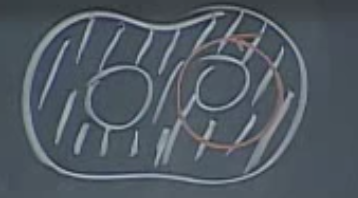
\includegraphics[height=3cm]{24_7.png}

Kirmizi ile gosterilen egri icindekilerin tamami $R$ icinde degildir. 





\end{document}
